\documentclass[10pt,conference]{cls/IEEEtran}
\usepackage{cite}
\usepackage{graphicx}
\usepackage[cmex10]{amsmath}
\usepackage{algorithm}
\usepackage{algorithmicx}
\usepackage{algpseudocode}
%\usepackage[caption=false]{caption}
\usepackage{subfig}
\usepackage{url}
\usepackage{booktabs}

% correct bad hyphenation here
\hyphenation{op-tical net-works semi-conduc-tor}


\begin{document}
%
% paper title
% can use linebreaks \\ within to get better formatting as desired
\title{CloudCache: An Alternative Way to Solve Hard Problems}

% author names and affiliations
% use a multiple column layout for up to three different
% affiliations
\author{
\IEEEauthorblockN{Jilong Liao}
\IEEEauthorblockA{Department of Electrical Engineering and Computer Science\\
University of Tennessee, Knoxville TN, 37996\\
Email: jliao2@utk.edu}
}

% make the title area
\maketitle


\begin{abstract}
In this document, an alternative approach is proposed to solve some very hard problems (e.g. 3-SAT and other NP-Complete problems) by using the power of cloud computing. The fundamental idea behinds this alternative approach is \emph{caching}. Since those NP-Complete problems have very large solution space, the cache requires a very large amount of storage. Cloud computing just provides such a convenience to support the necessity. In this document, we design and implement a framework which abstract the problem and solution as a \emph{key-value} object pair, such that its subproblems can also form some key-value object pairs. We store the key-value object pairs inside the CloudCache, and two simple cache APIs \emph{query()} and \emph{push()} are provided to support the caching operations. Besides, we simplify the problem solving framework as a \emph{kernel-solver} where people can define how they are going to solve a hard problem (like 3-SAT or k-coloring graph) using CloudCache framework very easily. To evaluate the performance of the framework, we deploy the framework to $6$ Amazon EC2 micro instances and try to solve $1,000,000$ 3-SAT problem instances (which is randomly generated) via the framework. The solution results are optimistic in terms of whether this caching approach could be an alternative way to solve hard problems.
\end{abstract}


\IEEEpeerreviewmaketitle

\section{Introduction}\label{sec:introduction}
Cloud computing has become one of the most powerful tools which could potentially help people solve some extremely hard problems. The computation and storage resource in the cloud are relatively cheap and convenient comparing to build something from the scratch. Besides, the public cloud vendors, like Amazon and Google, have made its own powerful computation and storage infrastructure available to the public via cloud computing service. Those cloud vendors provide either virtual machines or pre-defined cloud APIs to help people build application on top of their cloud very easy and fast.

By the booming time of cloud computing, people may have the chance to rethink of the way to solve some existing hard problems in computer science. The hard problems (usually belongs to the NP-Complete category like 3-SAT) often require exponential computation time to traverse the solution space in a brute-force manner. In addition, people may need to solve the same types of problems again and again in different instance. Some instances or subproblems possibly have been solved by others. Therefore, we come to the idea that \emph{cache the existing solutions to those problems and query the solutions before we solve any other problems}. 

One immediate challenge of this idea is the storage requirement. Even the same type of problem, e.g. 3-SAT, could have numerous problem instance, which may require several disks to store them, let alone we have many different types of hard problems. Cloud computing, at this point, could be a proper plagiarism because it is much less expensive to build a large scale storage and its management system. The other challenge is how we abstract the hard problems in a way that the platform we build could be more general to many different type of hard problems.

In this document, we propose \emph{CloudCache} framework which is built on top of general cloud computing platform and provides the interface to query, cache and solve hard problems in an easier way. The CloudCache framework abstracts the \emph{problem-solution} pair into \emph{key-value} objects, and uses some object storage system to cache existing problems and solutions. Further, the CloudCache framework provides a general problem solving interface \emph{kernel-solver}, so that the developer can easily write a problem's solution and solve it within the CloudCache's framework. CloudCache executes kernel-solver in a distributed way which tries to maximize the framework's problem solving throughput.

The rest of the document is arranged in the following way: Section~\ref{sec:design} describes the design and reasoning of the CloudCache framework; Section~\ref{sec:implementation} shows the implementations of the framework; Section~\ref{sec:evaluation} deploys the framework in Amazon EC2 and solves $1,000,000$ 3-SAT problem instances; Finally, we discuss some potential improvements and conclusion in Section~\ref{sec:conclusion}.

\section{Framework Design}\label{sec:design}
\subsection{The Problem-Solution Abstraction}
Many different types of hard problem we encounter have various input structure. For instance, 3-SAT problem input a logic expression while Clique problem needs a graph structure. Those different types of inputs brings the challenges to the CloudCache framework, because it is possible the CloudCache framework host many different types of problems and solutions and the cache query operation need to find the exact solutions for a certain problem. If we do not have a uniform structure for the all problems, the complexity in localizing problems and its solutions will be very large.

In CloudCache framework, we propose the general \emph{key-value} objects as the abstractions of problem-solutions where problems are the \emph{key} objects and solutions are the \emph{value} objects. To store the key-value objects in the general storage system (e.g. MySQL, Redis and MongoDB), we serialize the keys and values to strings. In this way, the general storage system can easily index, search and maintain the problems and its solutions regardless what type of problem it is.

For a specific problem, like the 3-SAT problem, the developers can define their data structure at their own convenience. The CloudCache framework's cache \emph{query()} and \emph{push()} APIs will first serialize the developer defined data structure when calling both APIs.

\subsection{Core System Design}
\begin{figure}
\centering
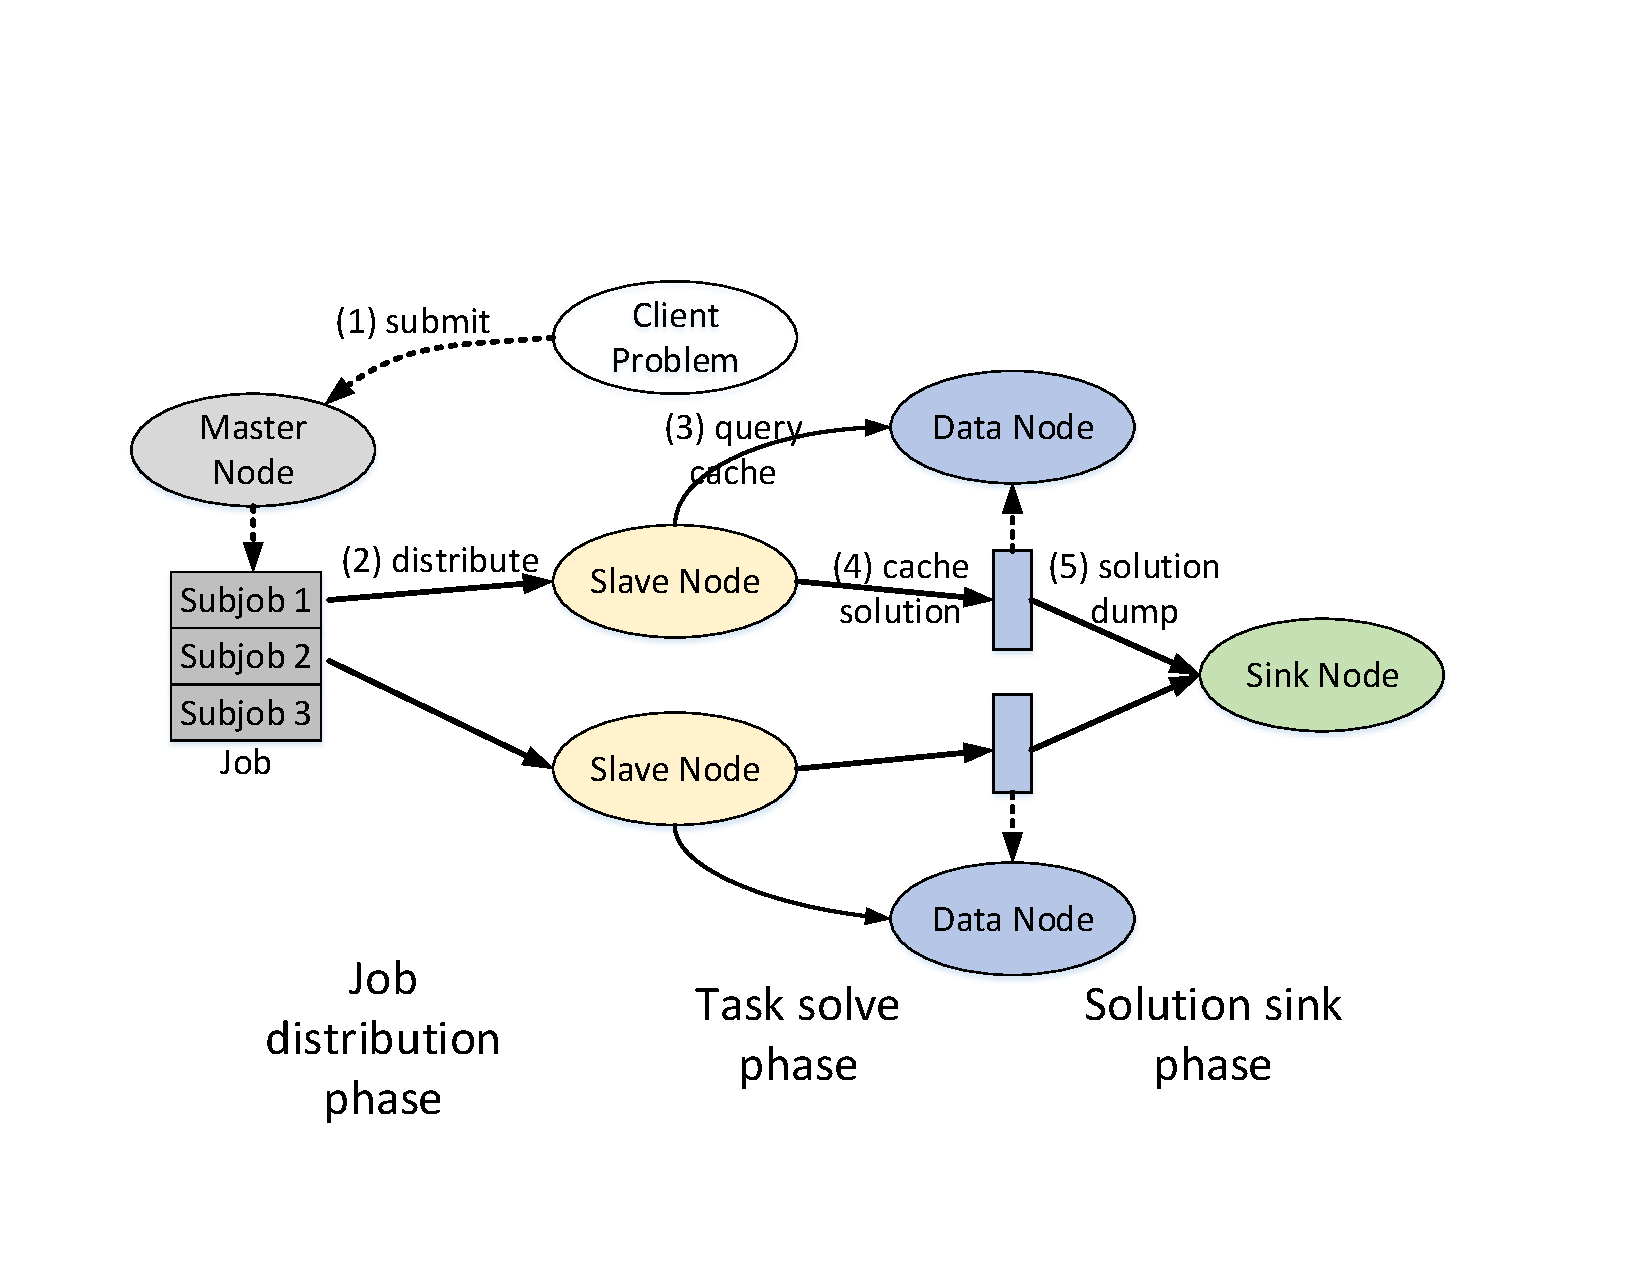
\includegraphics[width=0.5\textwidth]{pics/workflow.pdf}
\caption{The Logic Diagram of CloudCache}
\label{fig:logic}
\end{figure}

The CloudCache framework (Fig.~\ref{fig:logic}) includes four types of nodes and three computation phases in the cloud infrastructure. The nodes are \emph{Master Node}, \emph{Slave Node}, \emph{Data Node} and \emph{Sink Node}; the three phases are \emph{Job Distribution Phase}, \emph{Task Solve Phase} and \emph{Solution Sink Phase}. In addition, the \emph{Client Problem} exists outside of the cloud infrastructure which needs to be submitted into the CloudCache framework.

The Master Node is the central control component of the whole framework. It accepts the job submission from the client problem and split the the job into several subjobs. Those subjobs will later be distributed to different Slave Nodes. For each of the task in the subjob which the Slave Node is received from the Master Node, the Slave Node will initiate a \emph{kernel-solver} for the task. The kernel-solver is the single execution box defined by the developers for a problem which performs the cache query and solve functions. When the kernel-solver starts execution, it uses the \emph{query()} API to check if the current problem already has a solution in the CloudCache. The query API uses a \emph{hash} function to select the dedicated Data Node where a part of existing solutions are stored. Once the Data Node has been identified, the Data Node will response with a solution if the problem has been solved or a NULL value.

Whether the kernel-solver find the existing solutions or solve it by itself, the solution for the assigned problem will be cached in the Data Node, selected by the same hash function. We use a hash function to shard the queries because we consider the load balance of the Data Node which is much busier than Slave Node or Master Node in the system. In addition to cache the problem's solution, the solution needs to report to the Sink Node where the client program will come and retrieve the final results for all tasks in the job after the system finish the job. Note that we only have single Sink Node while the each kernel-solver will report its results to the Sink Node, the load at the Sink Node is significant which defects the whole system's throughput. Therefore, we have a small optimization that buffers the solution in each Slave Node until certain amount, then the Slave Node will report the buffered results together at once.

\subsection{Framework Generalness}
An expected design goal of CloudCache is the generalness, we want to make this framework to be a proper and simple approach to solve many different types of hard problems in the cloud. According to the design, only two things need to be defined by the developer before using the framework. First, the problem and solution's data structure; second, the kernel-solver of the problem, namely when to query the cache and when to solve the problem by itself. After finishing the two parts, the developer can submit a batch of problem as a job to the Master Node, where each problem is regarded as a task. Then the framework will start executing the batch job. In this section, we will show two hard problems' solution using CloudCache framework.

\subsubsection{3-SAT Problem}
The 3-SAT problem has an input of an boolean expression which contains many boolean variables' combinations in 3-conjunctive-normal-form clauses. For example, Eq.~\ref{eq:3-sat} shows an example 3-SAT problem which has $5$ boolean variables and has three clauses. For this problem, we use the expression vector as the key, but the vector is in a specific format. The boolean variable's index represents the variable itself in the vector, and the the index is set to be negative is the boolean variable has a ``not'' operator. The elements in expression are separated by a comma. Therefore, the \emph{key} for Eq.~\ref{eq:3-sat} is $[1,2,-3,2,3,4,3,-4,5]$.

\begin{equation}
Y = (x_1 \vee x_2 \vee \overline{x_3}) \wedge (x_2 \vee x_3 \vee x_4) \wedge (x_3 \vee \overline{x_4} \vee x_5)
\label{eq:3-sat}
\end{equation}

On the other hand, the solution of the problem is a vector of assignment, indicating each boolean variable's value as true or false. So for the 3-SAT problem instance in Eq.~\ref{eq:3-sat}, the \emph{value} is $[true, true, false, true, false]$. Once the key-value pair has been designed, we can move on to the \emph{kernel-solver} part.

The kernel-solver has two stages, the first stage is to check if the expression or any subexpression has been solved. We use a linear scan to do it by moving the head clause and check the subexpression between the head clause and the end one. For the example in Eq.~\ref{eq:3-sat}, we will check Eq.~\ref{eq:3-sat1},~\ref{eq:3-sat2},~\ref{eq:3-sat3}. If any of the subexpression has been solved, we will retrieve its solution then validate if the assignment can satisfy the whole expression. If so, we do not need a brute-force method to solve it again but just return the assignment in the cache. Otherwise, the brute-force method has to be run and we need to store the solved assignment in the cache. The two simple APIs to query and store key/value in the CloudCache make the operations very easy to do.

Note that we do not enumerate the possible combination of clauses in the expression to query the cache. The major reason is that most of the 3-SAT is not as hard as we may expect, thus the enumeration process may cost more time than a simple brute-force try. Besides, we cannot estimate the cache hit ratio for a clause combination ahead which may make the solution even slower as well.

\begin{equation}
Y = (x_1 \vee x_2 \vee \overline{x_3}) \wedge (x_2 \vee x_3 \vee x_4) \wedge (x_3 \vee \overline{x_4} \vee x_5)
\label{eq:3-sat1}
\end{equation}
\begin{equation}
Y = (x_2 \vee x_3 \vee x_4) \wedge (x_3 \vee \overline{x_4} \vee x_5)
\label{eq:3-sat2}
\end{equation}
\begin{equation}
Y = (x_3 \vee \overline{x_4} \vee x_5)
\label{eq:3-sat3}
\end{equation}


\subsubsection{k-coloring Problem}
The graph's k-coloring problem is to find a color assignment strategy that mark the vertex of the graph so that no adjacent vertex share the same color by using no more than k different colors. The problem is also a classic NP-Complete problem, the exact solution is a brute-force one by enumerating the $k^n$ assignments and validate them.

Similarly, we first need to abstract the problem-solution pairs. For the problem, we use a matrix $\mathbf{R}_{n\times n}$ to represent the graph which is the \emph{key}, and the \emph{value} is the color assignment vector $\mathbf{a} = [a_1, a_2, ..., a_n]$ where $n$ is the number of vertex in the graph.

The kernel-solver is also using a linear scan to all the vertices. For each vertex, we remove the edges connected to the vertex, then we have a new adjacent matrix $\hat{\mathbf{R}}_{(n-1)\times (n-1)}$ which is actually a subgraph of the original one. For this subgraph, we query the CloudCache to retrieve the existing color assignment. If success, we need to validate the assignment by enumerating the color of the removed vertex combining with the existing solution to see if the complete assignment can fit into the original graph. If so, we can cache the solution; if not, we continue removing another vertex in $\mathbf{R}_{n\times n}$ until we scan all the vertices one time. If cache is not working at all, the brute-force solver is triggered. 

\section{Implementations}\label{sec:implementation}
In this section, we describe the implementation details of the CloudCache framework. Specifically, we will use the 3-SAT problem as the sample to illustrate the infrastructure, software architecture, and programming interface.

\subsection{The CloudCache Infrastructure}
As is shown in Fig.~\ref{fig:system}, the infrastructure in the cloud consists of four different types of nodes: Master Node, Slave Node, Data Node and Sink Node. Outside of the cloud infrastructure, we have a Client which will submit the job to the Master Node. After the job is done, the Sink Node will push the job results to the Client.

The Master Node runs a multi-threaded TCP server, waiting for the job submitted from the Client. We consider the possibility of concurrent job submission from the clients, then the multi-threaded server is required. However, we do not optimize the server's performance under some pressure test. The Slave Node is also a multi-threaded TCP server, but once the Slave Node receives the job distributed from the Master Node, it will fork a worker thread to execute every task in the job. We do not fork multiple threads for each task because we do not want the first arrive job's tasks overwhelm the Slave Node (it is possible for Slave Node to run different jobs concurrently).

The Data Node is a tricky part in the system, because we combine the Slave Node and Data Node together in single physical machine. So a machine in the cloud will both solve the problem and host the data. We use hash function to shard the solution's cache choice. The reason for this implementation is that we want to maximize the possibility of local cache query and avoid unnecessary and frequent remote cache check which is very time consuming. In addition, we do not choose SQL database such as MySQL as the local storage system, but use some NoSQL techniques such as Redis~\cite{macedo2011redis} to be the persistent data storage. We believe the NoSQL techniques have much better performance to manage the key/value objects.

Finally, the Sink Node is the one to collect all the results and provide the final job result to the Client. To avoid the Slave Node's highly frequent task report, we buffer the report at the Slave Node until the buffer is full. This small optimization reduce the load of Sink Node, and increase the Slave Node's efficiency as well (task reporting blocks the Slave Node moving forward).

\begin{figure}
\centering
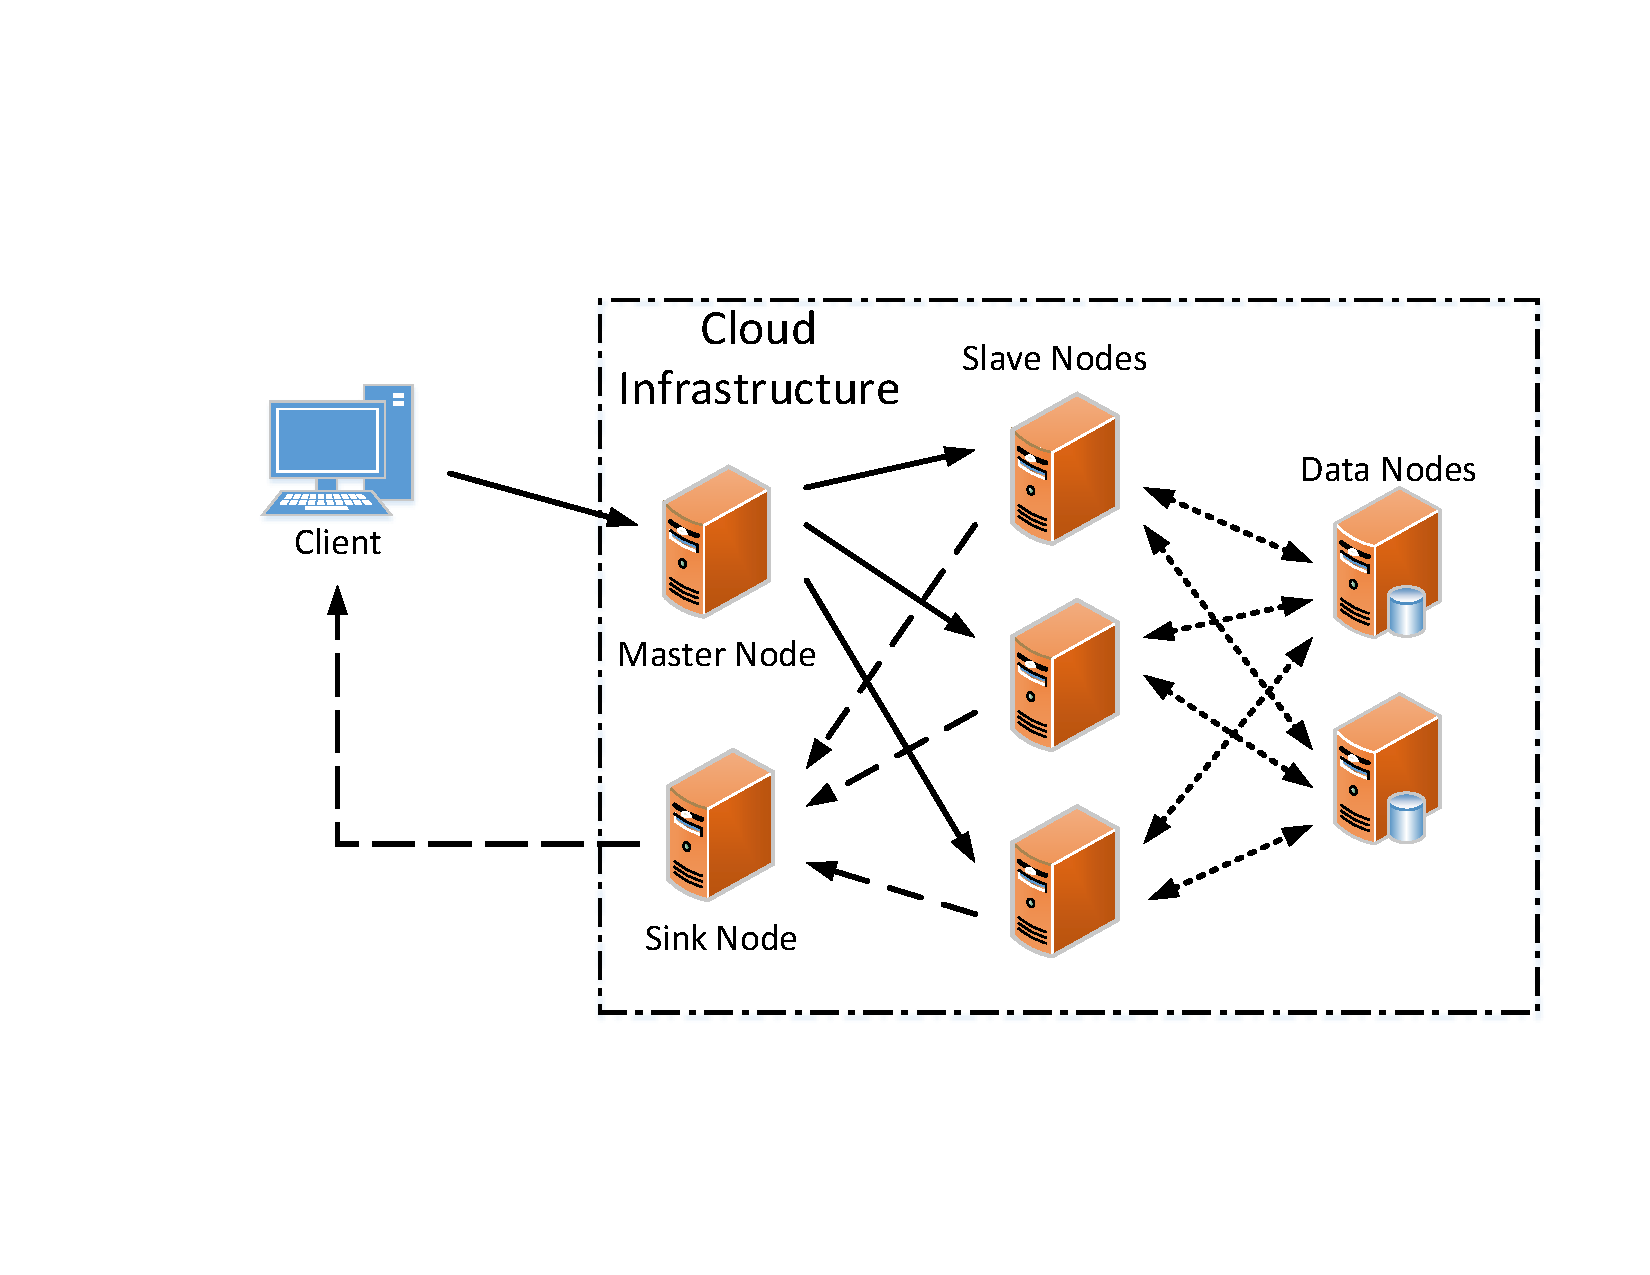
\includegraphics[width=0.5\textwidth]{pics/cloud-cache-arch.pdf}
\caption{The CloudCache System Diagram}
\label{fig:system}
\end{figure}

\subsection{Software Architecture}
We use Python as the language to implement the system. It consists of seven major modules in the source code\footnote{Source code is hosted on Github: https://github.com/little-eyes/cloud-cache.git}.

\begin{itemize}
\item master.py. This module is the component to start a Master Node, which contains a multi-threaded TCP server, job class and some global variables for bookkeeping and statistics.

\item slave.py. This module is the component to start a Slave Node. It includes a multi-threaded TCP server as well, and a job execution handler and some statistic variables.
\item sink.py. The Sink Node module which receives the accumulated task report and dump the solutions to disk. After the job finished, the Client can come to retrieve the results.
\item kernel.py. The core module to kernel-solver. A developer should define a class to solve the problem, then the Slave Node will call the kernel-solver based on the configuration.
\item tools.py. It defines many helper class to help simplify the architecture like JobDispatcher, etc.
\item configure.py. The place is used to define any global configuration details, for instance, the Master Node, Slave Node, Data Node and Sink Node.
\end{itemize}

For the Redis server, it has to be deployed before running any module in the Data Node. Since we combine the Data Node and Slave Node into one physical machine, the Redis server is running as a service in the operating system.

\subsection{Programming Interface}
Two important programming interface in the CloudCache is in the tools.py module. The two APIs are \emph{tools.PersistentStorageManager.query(key)} and \emph{tools.PersistentStorageManager.push(key, value)}. 

A developer can call these two APIs to simply the cache operations in the implementation of kernel-solver. The kernel-solver is an abstract name, however, in practice, a developer needs to implement the solver class. For example, the 3-SAT problem, we implement \emph{BaseKernel3SAT} and \emph{CloudCacheKernel3SAT} classes which will be instantiated in job execution handler. Again, the developer does not need to pay additional attention to the data structure of key and value, because the two APIs above will serialize the key and value first before conducting cache operations.

\subsection{Implementation Optimizations}
After we implement the first version, we do not find too much advantages of the CloudCache framework. Thereafter, we analyze the code we write, and we realize the interaction between the Slave Node and Data Node are too frequent during the problem solving phase, which is reaching the benchmark upper bound of the Data Node. Each query and push operations costs more time than it should be. Therefore, we use a pipeline technique to solve the problem. Every time the problem is fully solved, either through cache query or brute-force, we put the result key-value pair into a pipeline. When the pipeline has certain number of solutions need to be cached in the cloud, we execute the whole pipeline once. This brings a decent performance gain for the CloudCache framework.

\section{Evaluations} \label{sec:evaluation}

\section{Conclusion}\label{sec:conclusion}
In this document, we describe the design and implementation of CloudCache framework. Through the evaluation, we find that the advantages of CloudCache framework has larger margin for the hard solving problem instances. We also look into the generalness of the framework by designing the solutions for the \emph{k-coloring} problem in the graph. The the solution paradigm fits into the problem very well, which reinforce the advantages of CloudCache framework. Finally, the system performance in CPU and network-in/out evaluation provides us a good fingerprints of the CloudCache framework as a whole.




\bibliographystyle{IEEEtran}
\bibliography{reference}  % sigproc.bib is the name of the Bibliography in this case

%\bibliographystyle{IEEEtran}
%\bibliography{ref}


% that's all folks
\end{document}


